\part{Projektdokumentation}

\chapter{Anforderungs- und Problemanalyse}
Aufgabe der Anforderungsanalyse in diesem Projekt war es herauszufinden welches Problem die Kundin mit der zu entwickelnden Software lösen möchte. Dafür wurden Interviews mit dem Kunden durchgeführt und entsprechende Ergebnisse mit Hilfe von Audioaufzeichnung, Mitschriften und Fotografien protokolliert. Zur detaillierten Beschreibung einzelner Abläufe des Systems wurden Kreativtechniken wie das Zeichnen verschiedener Szenarien an einem Whiteboard sowie die manuelle Simulation des Fahrstuhles mit einem aus Pappe gefertigten Modells durchgeführt.
\begin{figure}[hbt]
\centering
\subcaptionbox{Skizze der Fahrstuhlsimulation am Whiteboard}[0.49\linewidth]
{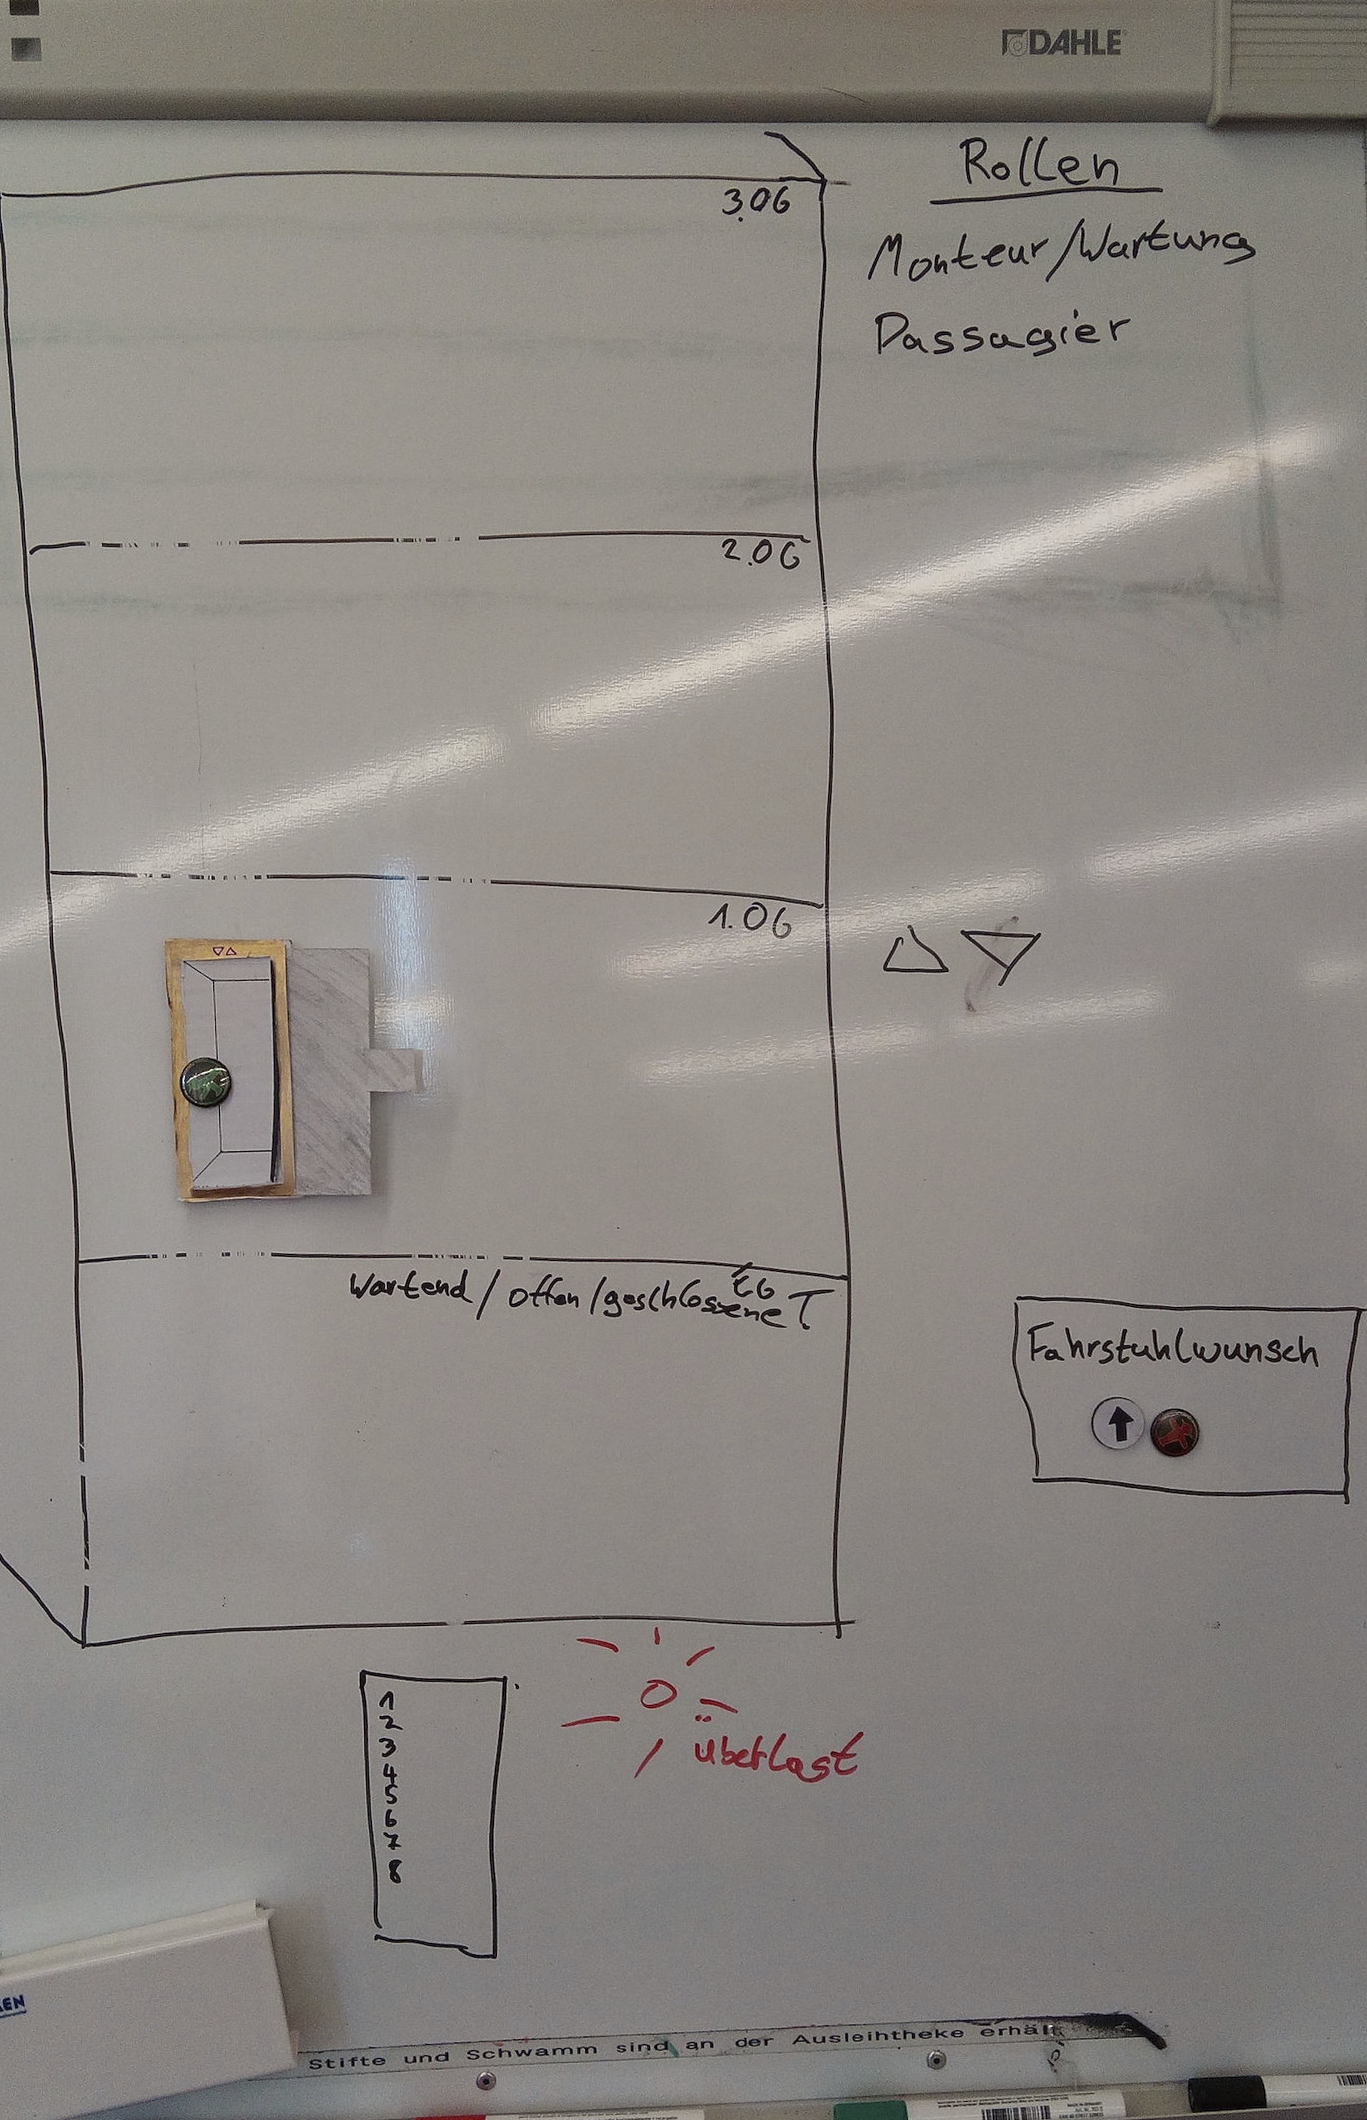
\includegraphics[height=8cm]{images/kundengespraech1.jpg}}
\subcaptionbox{Modell des Fahrstuhles}[0.49\linewidth]
{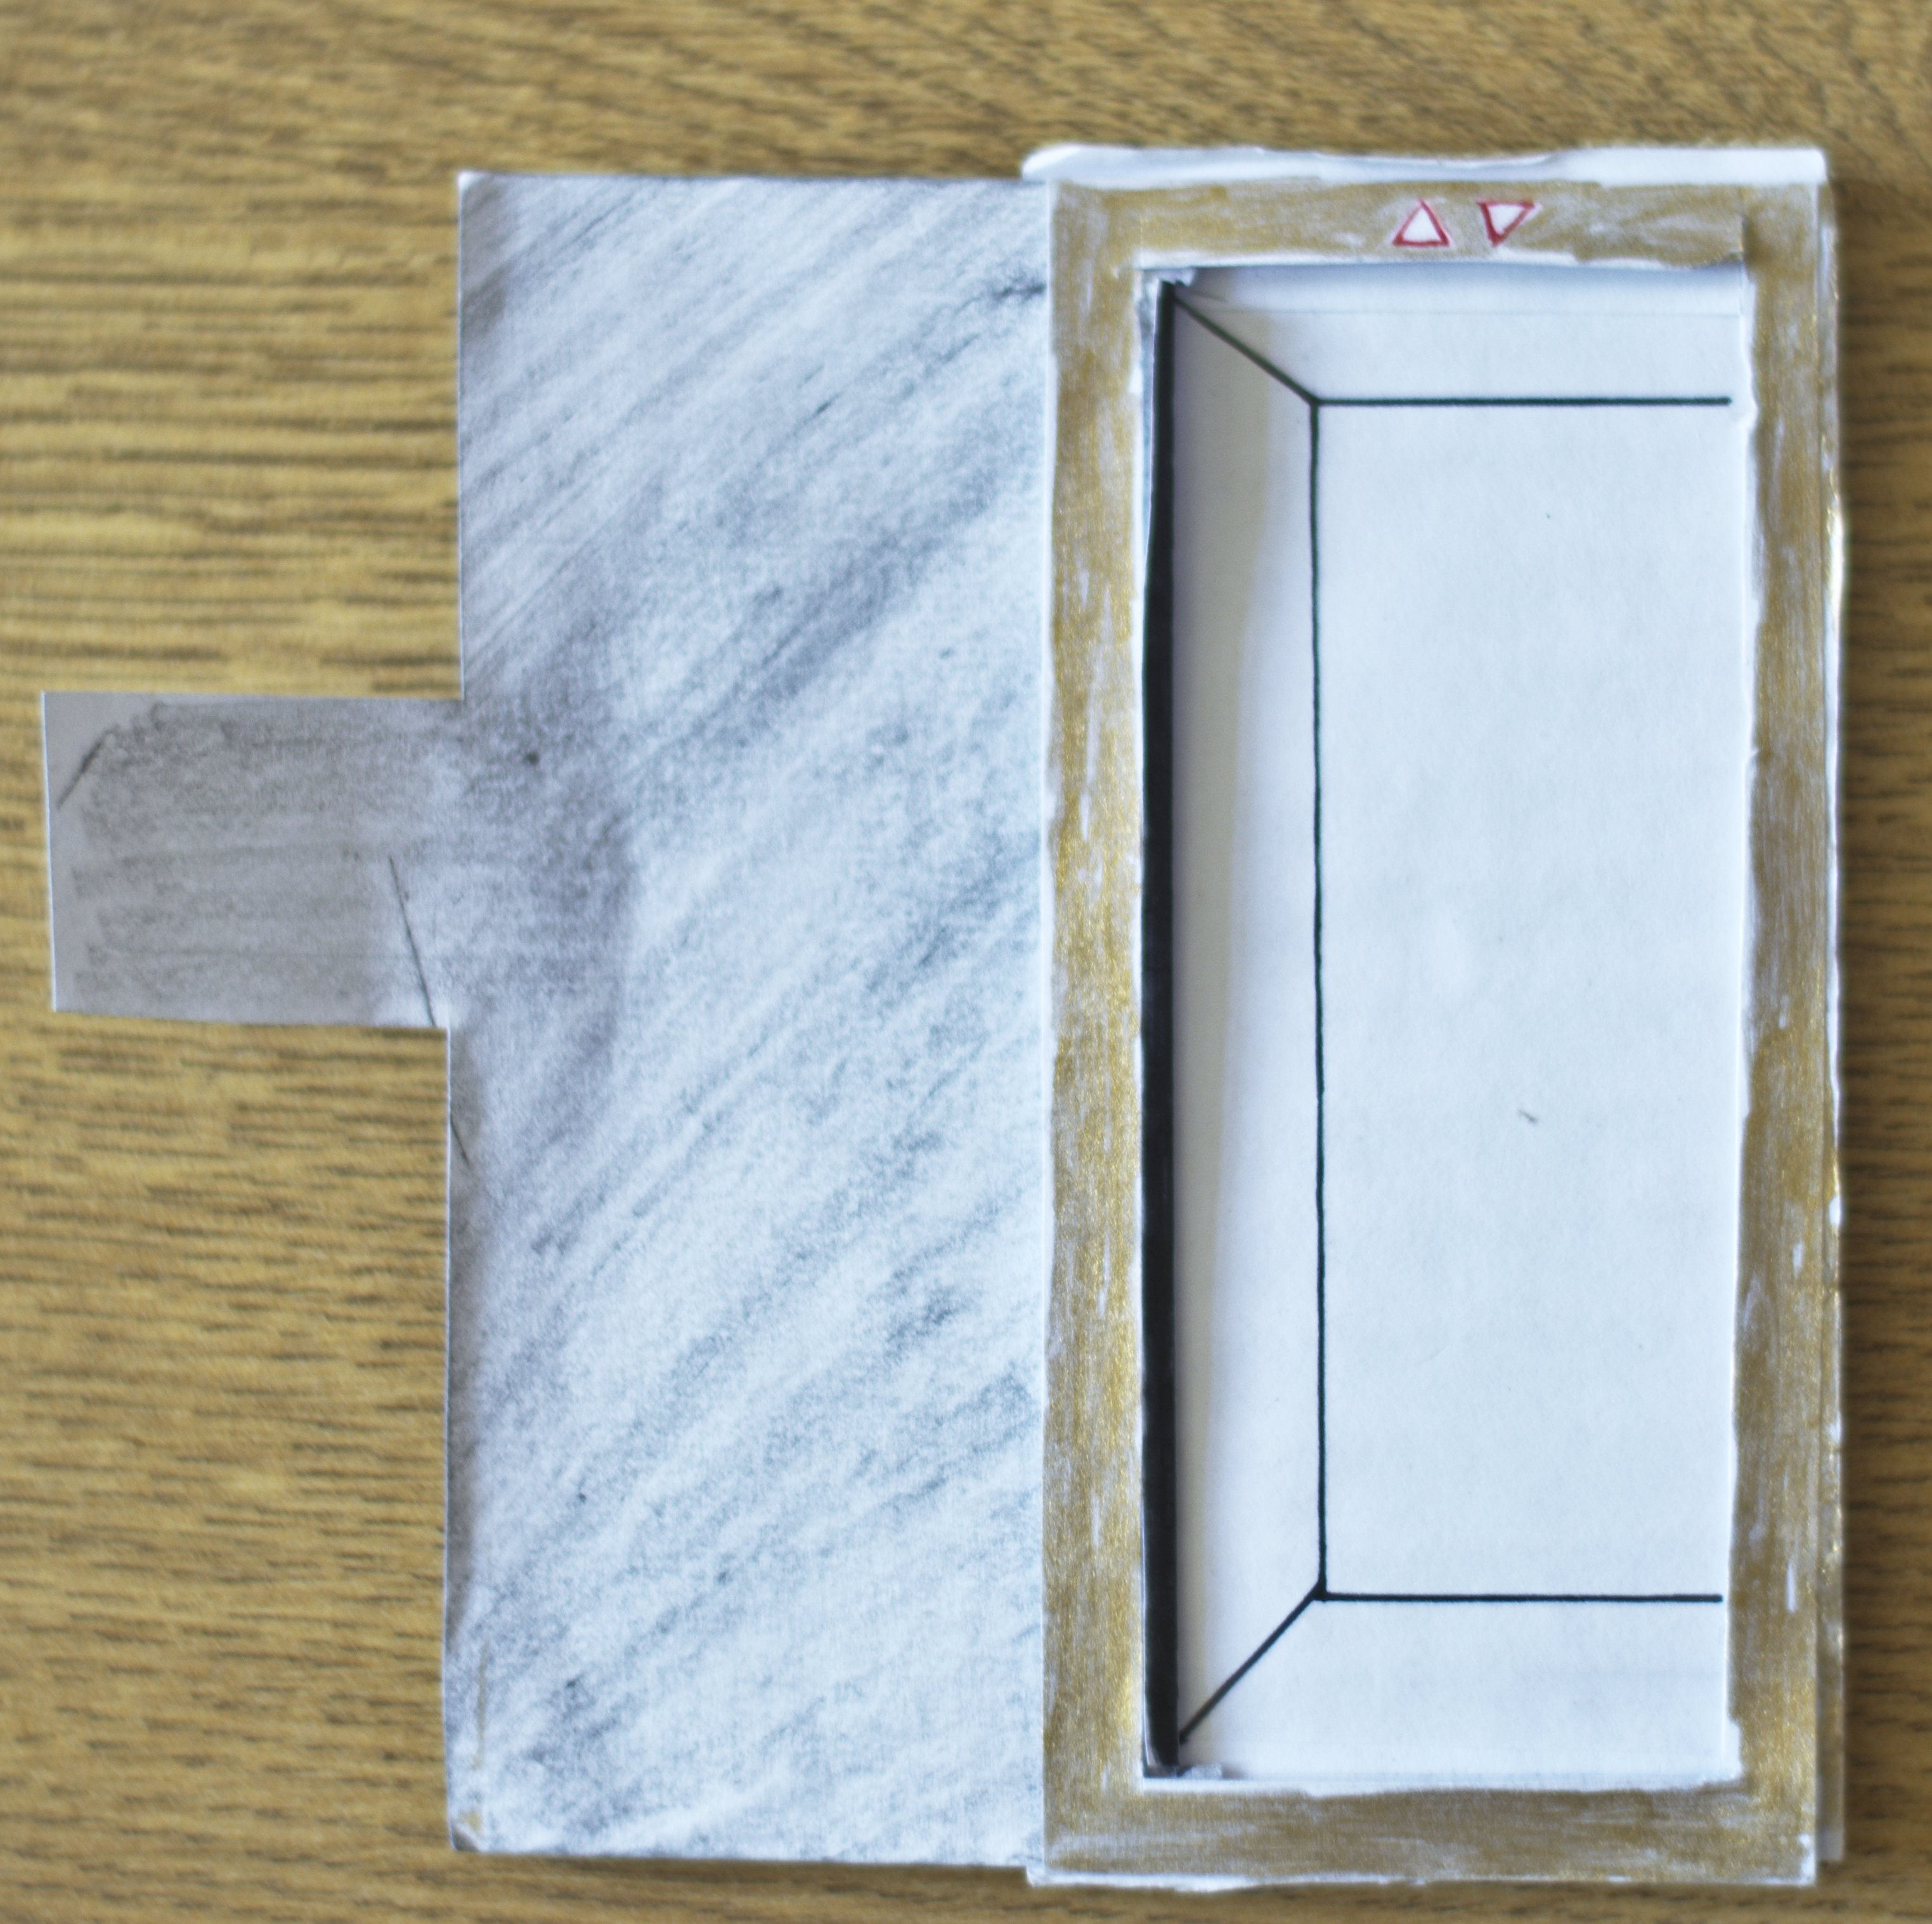
\includegraphics[height=8cm]{images/pappfahrstuhl.jpg}}
\caption{Kreativtechniken zur Anforderungsanalyse}
\end{figure}
Die folgenden grundlegende Fragen waren im Laufe der Analyse zu klären:
\begin{itemize}
	\item Wie viele Fahrstühle sollen verwendet werden können?
	\item Wie soll das Gebäude beschaffen sein?
	\item Welcher Algorithmus soll verwendet werden?
	\item Gibt es Schnittstellen zu anderen Systemen?
\end{itemize}
Weiterhin musste festgelegt werden ob die Priorität des Systems auf der Simulation oder auf einer möglichst realitätsnahen Umsetzung eines Liftes liegt. Im Laufe der Analyse und Modellierung entsprechender Anwendungsfälle wurde ersichtlich, dass das System sich aus zwei Teilsystemen, der \textbf{Fahrstuhlsteuerung} und der \textbf{Fahrstuhlsimulation} zusammensetzt, deren Anforderungen getrennt voneinander beschrieben werden mussten.\\
Eine Besonderheit des Systems ist dabei die Umgebung in der es eingesetzt werden soll, der Lehrbetrieb an einer Hochschule. Daraus ergaben sich spezielle Anforderungen, wie das Anzeigen der Zustandsübergänge, die gesondert betrachtet werden mussten.

\paragraph{}Vor allem aus den letztgenannten Anforderungen formte sich während der Analyse relativ früh unsere Vision einer Anwendung, welche in einer zweigeteilten Sicht Fahrstuhl und Zustandsdiagramm nebeneinander darstellt. Zusätzlich sollten Zustandsübergänge und aktive Zustände durch Animationen kenntlich gemacht werden.

\paragraph*{}Die Resultate der Analysephase, alle Anwendungsfälle und Vereinbarungen mit der Kundin wurden am Ende im Pflichtenheft festgehalten, welches als eigenständiges Dokument am Ende der Phase an die Kundin überreicht wurde. Diese Dokument war im weiteren Verlauf des Projektes ein zentrales Maß bei regelmäßigen Treffen und Evaluationen.



\chapter{Software-Entwurf}
Nach der Festlegung von Anforderungen und der Beschreibung der Funktionalitäten der Fahrstuhlsimulation war der nächste Schritt der Entwurf der internen Struktur. Wir näherten uns dieser Problemstellung von außen und erhöhten bei steigender Tiefe die Granularität. Dies bedeutete zunächst, die geeignetste Rahmen-Technologie festzulegen, welche die Anforderungen unseren Kundin am besten erfüllen konnte.

\section{Technologie}
Die Wahl der verwendeten Technologie fußte prinzipiell auf drei Hauptpunkten, erstens unserer Vision einer optisch ansprechenden Anwendung, welche das Zusammenspiel von System und dessen Zuständen visualisiert. Zweitens einer möglichst umfassenden Kompatibilität zu verschiedenen Plattformen und drittens der verfügbaren Zeit zur Realisierung aller Anforderungen. In Anbetracht der kurzen Projektzeit entschlossen wir uns zunächst eine Vorauswahl zu treffen. Diese sollte ausschließlich Technologien enthalten, auf deren Gebieten bereits Erfahrungen im Team vorhanden waren. Nach kurzer Diskussion ergaben sich als Möglichkeiten die Nutzung von \textsc{C++}, \textsc{Java} oder \textsc{Web-Technologien} wie \textsc{Javascript}.

\paragraph*{}Nach reiflicher Überlegung und wiederholter Rücksprache mit unserer Kundin erschienen uns \textsc{Web-Technologien} am geeignetsten um alle Anforderungen in der zur Verfügung stehenden Zeit umzusetzen. Die Vorteile dieser Technologien, welche unsere Entscheidung maßgeblich beeinflussten, waren folgende:

\begin{enumerate}
	\item Sie ermöglichten uns größtmögliche Plattform-Kompa\-tibilität, da unser Produkt einerseits als Cross-Plattfom-Anwendung und andererseits als Web-Site veröffentlicht werden können.
	\item Mit den modernen Mitteln des Web-Designs war es uns möglich die hohen grafischen Anforderungen an das Software-System in derart kurzer Zeit umzusetzen.
\end{enumerate}

Gebündelt und verwendet wurden diese Möglichkeiten durch modere Werkzeuge der Web-Entwicklung wie \textsc{ReactJS}\footnote{\url{http://facebook.github.io/react/}}, \textsc{nodeJS}\footnote{\url{https://nodejs.org}}, \textsc{bower}\footnote{\url{http://bower.io}} oder \textsc{grunt}\footnote{\url{http://gruntjs.com}}. An dieser Stelle verweisen wir auf die entsprechenden Stellen der Entwicklerdokumentation.

\section{Algorithmus}
Die wesentliche Funktionalität sowie der Algorithmus des Systems lassen sich in
dem Zustandsdiagramm abbilden. Um das bestmögliche Ergebnis zu erhalten haben
wir verschiedene Versionen des Diagramms entworfen und diese in Gruppentreffen diskutiert und überarbeitet.
\missingfigure[figwidth=\textwidth]{Zustandsdiagramm ggf. mehrere Versionen}

\paragraph{}Diese Vorauswahl bestand
Für die technische Umsetzung der Zustände in ausführbaren Quellcode ergaben sich folgende Entwurfsmuster:
\todo{Wir müssen aufpassen, dass wir eine klare Trennung zwischen Entwurfs-spezifischen Inhalten im Entwicklerhandbuch und hier vornehmen.}
\subsection*{State Design Pattern}
Vorteile, Nachteile, warum haben wir uns dageben entschieden?
\todo{Nachteile: großer Overhead, da hier nur 3 Zustände vorkommen, jedoch die Zustandsübergänge komplex sind}
\subsection*{Zustandstabelle}
\todo{nicht sinnvoll zwecks erweiterbarkeit/wartbarkeit}

Die eigentliche Herausforderung des Systems besteht nicht in den Zuständen, sondern in den Zustandsübergängen, da der Fahrstuhl bis auf wenige Ausnahmen wie von \textbf{Idle} nach \textbf{Stop} in jeden beliebigen Zustand springen kann.
\subsection*{Event Emitter}
\subsection{Observer Pattern}

\chapter{Qualitätssicherung}
\section{Allgemein}
Der Standard ISO/IEC 25000:2014 welcher als Einleitung zu genormten Methoden der Qualitätssicherung in der Software zu verstehen ist, definiert diese als "`Systems and Software Quality Requirements and Evaluation (SQuaRE)"'\cite[Foreword]{ISO25000}. Festzustellen ist: Der ISO25000 ist für einen Norm relativ jung ist und löst zwei Vorgänger, welche die Themen Softwarequalität bzw. Anforderungsanalyse (ISO/IEC 9126) und Software Evaluierung bzw. Test (ISO/IEC 14598) überwiegend getrennt behandeln ab. Neben der Motivation der Vermeidung von Redundanzen und Inkonsistenzen zwischen den zwei Normen, ist es Meinung des Autors, dass sich hierbei die Erkenntniss der notwendigen Verzahnung der beiden Teilgebiete zeigt. So werden z.B. im \textit{test driven development} idealerweise die Anforderungen direkt zur Software-Evulation benutzt.

\paragraph*{}Aus der Definition
\begin{quote}\label{PD_SQ}
software quality
capability of software product to satisfy stated and implied needs when used unter specified condidtions
\end{quote}\cite[4 Terms and definitions]{ISO25000}
lässt sich somit die umfassende Qualitätssicherung aufteilen auf
\begin{enumerate}
\item Einwirkung auf Anforderungsanalyse
\item Evaluation während und nach der Umsetzung
\end{enumerate}
da sich Softwarequalität nach obiger Definition rein auf die bereits eruierten Anforderungen und Bedingungen stützt, wie Gesamtzufriedenheit des Nutzers allerdings nur dann erreichen lässt, wenn diese Vorbetrachtung bestmöglich durchgeführt wurde.
\section{QS Anforderungsanalyse}
Zu Beginn des Projekts wurde beim der Erstellung des Pflichtenheftes auf saubere und eindeutige Formulierungen geachtet, da Probleme in dieser Phase die größten Auswirkungen auf die Zufriedenheit des Nutzers besitzen.\\
Desweiteren wurde durch erneuten Vergleich der Anforderungen mit Kundenprotokollen und Aufgabenstellung sowie Prüfen auf Inkonsistenzen assistiert.

Als qualitätsunterstüzende Maßnahme wurden die Anforderungen möglichst auf sogenannte Issues, also Stichpunkte und Meilensteine in einem Projektmanager, abgebildet.
\section{QS Umsetzung}
\subsection{Allgemein}
\begin{itemize}
\item Konvetionen
\item Testregime
\end{itemize}
\subsection{Konventionen}
\todo{Traceabillity hinzufügen -> jede Anforderung muss im Quellcode durch einen commit oder ähnlich nachverfolgbar sein}
\subsection{Codekonventionen}
Um bei der Arbeit in der Gruppe an einer gemeinsamen Quellcode-Basis einen hohen Qualitätsstandard der Quelltexte zu bewahren, wurden Konventionen festgelegt die den Entwicklern vorgeschrieben haben wie z.B. Methoden und Variablen benannt werden sollen. So wurde festgelegt, dass
\begin{itemize}
 \item Methodennamen in camelCase Notation zu bezeichnen sind
 \item im Quelltext keine nachgestellten Leerzeichen\footnote{engl. trailing whitespace} vorkommen dürfen
 \item keine Quelltextzeile länger als 80 Zeichen ist
 \item private Variablen mit einem Unterstrich gekennzeichnet werden
\end{itemize}

\todo{Code Konventionen, statische Codeanalyse}
\subsection{Test}
Für die automatischen Tests wurde das Testframework Jasmine\footnote{http://jasmine.github.io}

\subsubsection{manuelle Testfälle}
\subsubsection{automatisierte Testfälle}

\chapter{Team-Organisation}
\section{Gruppenarbeit}
Um das Zusammenarbeiten in der Gruppe einfacher zu gestalten wurden verschiedene Technologien eingesetzt.
Zu finden von Terminen für Meetings wurde Doodle\footnote{\url{www.doodle.com}}  verwendet. Für die Kommunikation in der Gruppe Slack\footnote{\url{https://slack.com/}}.
\todo{Hier muss hin warum wir uns für JS und Co entschieden haben.}
\section{Verwendete Werkzeuge}
\section{Resümee}

\bibliographystyle{plaindin}
\bibliography{projektdokumentation}
